\documentclass[12pt]{article}

\usepackage{amsmath, amssymb, amsthm, graphicx, fancyhdr, textcomp, enumerate, diagbox, tcolorbox, esvect, tikz, adjustbox}

\graphicspath{{./images/}}

\usepackage{halloweenmath, tikzsymbols}

\newcommand{\R}{\mathbb{R}}
\newcommand{\Z}{\mathbb{Z}}
\newcommand{\C}{\mathbb{C}}
\newcommand{\N}{\mathbb{N}}
\newcommand{\Q}{\mathbb{Q}}
\newcommand{\Arg}{\mbox{Arg}}
\newcommand{\Log}{\mbox{Log}}

%geometry/topology
\newcommand{\bndry}{\partial}


\newcommand{\infsum}{\sum_{n = 1}^{\infty}}
\newcommand{\pf}{\fbox{proof}}
\newcommand{\cor}{\fbox{corollary}}

\theoremstyle{definition}

\newtheorem*{definition}{Definition}
\newtheorem{lemma}{Lemma}
\newtheorem{theorem}{Theorem}
\newtheorem{corollary}{Corollary}
\newtheorem{proposition}{Proposition}
\newtheorem{remark}{Remark}
\newtheorem{conjecture}{Conjecture}
\newtheorem{example}{Example}

\newcommand{\inv}[1]{#1^{-1}}

\title{Modern Geometry}
\author{August}

\begin{document}

\maketitle

\section{Problem 5.3}


\begin{proposition}
The minimum number of edges in the medial axis of a convex polygon $P$ with $n$ vertices is $n$.
\end{proposition}
\begin{proof}
To see this, note that every vertex of the polygon will correspond to one angle bisector, and hence one edge of the medial axis. Finally, it is always possible to actually achieve this lower bound by considering the regular polygon with $n$ vertices. 
\end{proof}

The interesting part is that the maximum number of edges is $2n-3$. The proof of this also gives us what I consider to be a pretty remarkable result about binary trees and medial axis.

This general lemma about trees will be useful for us.
\begin{lemma}
Let $T$ be a binary tree with $n\ge 2$ leaves. Then the number of edges is $2n-3$. 
\end{lemma}

\begin{proof} The proof is by induction. First note that for $n = 2$ leaves, we have $2(2) - 3 = 1$ edge, and the graph with two vertices clearly satisfies this requirement.\\

Now suppose for $n > 2$ we have that any binary tree with $n$ leaves satisfies the formula $E = 2n-3$. Let us now consider a binary tree with $n+1$ leaves. select one leaf. Then this leaf, and another, are "ancestors" of another vertex. Removing these two leaves, we turn their ancestor into a leaf, and have a graph with $n$ leaves (since we have lost two and gained one leaf in the process of removing these two. Therefore we have $2n-3$ edges in this graph. Adding back the two leaves, we gain two more edges, giving us $2n-1 = 2(n+1) - 3$, so the induction step works.
\end{proof}

\begin{lemma}
The non-leaf vertices of the medial axis tree of a convex polygon are of degree at least three.
\end{lemma}

\begin{proof}
This can be proven from the algorithm which constructs the medial axis of a convex polygon. We proceed by induction. In the case of the triangle, this clearly holds. Now suppose it holds for any convex polygon with $n-1$ edges. Let $P$ be a polygon with $n$ edges. Pick two adjacent vertices whose angle bisectors meet "first" at some point $v$. Extending the adjacent edges to the vertices to meet at some other point $p$. Then the rest of the edges of the medial axis are part of the medial axis of the larger $n-1$-gon. As a result, we can apply the induction hypothesis to the remaining vertices of the medial axis of $P$. Moreover, there will be a third edge at $v$ which is the angle bisector at $p$. Hence $v$ has degree $3$. This covers all of the vertices. 
\end{proof}

\begin{lemma}
Let $P$ be a polygon such that some medial axis vertex is of degree greater than $3$. Then there exists a polygon $P'$ with $n$ vertices such that the medial axis tree of $P'$ has more edges than $P$, while $M(P')$ has no vertices of degree more than $3$.  
\end{lemma}


\begin{proof}
Given such a polygon $P$, let $v$ be the non-leaf vertex which has degree greater than $3$. Chose a line $\ell$ which passes through $v$ so that both sides of $\ell$ contain at least two of the edges of $v$, and let $S_1$ and $S_2$ be corresponding partitions of the edges adjacent to $v$. Because the medial axis tree does not cross itself, it follows that these partitions $S_1$ and $S_2$ give a partition of the vertices of $P$ into two sets which are connected by edges of $P$. Now draw a line through $v$ which cuts the polygon $P$ into two sections, respecting the partition of the vertices of $P$. Translate the two partitions away from each other by some distance, and in a direction orthogonal to this line. This will give us a new polygon $P'$, which will have all the same medial axis tree except for adding one and a new vertex, dividing the edges adjacent to $v$. Since on both sides there is at least two less adjacent edges, and since we have only added one edge, we have lost at least one edge, for both of these vertices. Repeat this process for each such edge $v$ until we have only vertices of degree $3$ or less. At each step, we have gained one edge in total, and lost none. Moreover, we have kept the same number of vertices of the polygon.
\end{proof}

\begin{corollary}
Since the nodes of the medial axis are of degree at least three, or are leaves (which are the vertices of the polygon), it follows that $2n-3$ is an upper bound for the number of edges in the medial axis tree of a convex polygon with $n$ vertices. Still, it remains to show that this upper bound is actually achieved.
\end{corollary}

\begin{lemma}
It is always possible to construct a polygon $P$ with $n$ vertices so that the non-vertex vertices (the nodes which aren't leaves) of the medial axis tree are of degree  $3$ (is a binary tree). 
\end{lemma}

\begin{proof}
We proceed by induction. First, in the case of the triangle, we have only one non-vertex vertex (lol), and it has degree $3$. Now suppose that for some $n-1$, it is possible to construct some polygon $P$ so that all of the non-leaf vertices are of degree $3$. Now select any vertex $v$ of $P$. Cut edges adjacent to $v$ at some point closer to $v$ than the bisector of the edge, and create a new polygon $P'$ by truncating $P$ at these points. Then we have acquired one more vertex. Moreover, new edges that are the angle bisectors of the newly formed vertices will intersect each other before intersecting elsewhere, as we have constructed them so as to be closer together. Hence the resulting polygon $P'$ has all of its non vertex vertices of its medial axis of degree $3$, and the polygon has $n$ vertices.
\end{proof}

As an easy corollary, we have an upper bound which is actually realized for the number of edges in a convex polygon with $n$ vertices. I conjecture that it is the same for the general case (dropping the convexity requirement).

\begin{remark}
One remarkable consequence of this result is that every binary tree is the medial axis of some polygon!
\end{remark}

\section{5.4}

Suppose we have house which is a $W\times L$ rectangle, where $L> W$, so that the roof is the medial axis polyhedron of the rectangle. If we have "rain" falling onto the roof, the ratio of the rain which falls of each edge of the roof will be precisely the area of the region bounded by the medial axis of the rectangle (viewed as a polygon by projecting onto the $xy$ plane. \\
Since the angle bisector at each of the vertices comes out from $L$ at exactly a 45 degree angle, the two angle bisectors meet at exactly the midpoint of $W$, so we have a triangle with base $W$ and height $W/2$. Hence the area is bounded by either of the sides of length $W$ (labelled $R_1$ and $R_2$ in the diagram) is $W/4$. Moreover, adding these two areas together, and noting that the area of the rectangle is $WL$, as well as the fact that the two regions are equal, we find upon solving the equation that the remaining two areas are $W\frac{(L - \frac{1}{2})}{2}$. \\

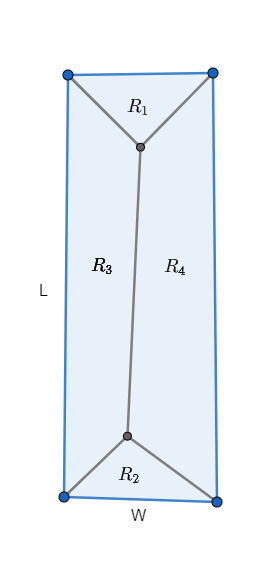
\includegraphics[scale=0.4]{polygon_roof_base.png} 

Therefore, for either of the sides of length $W$ ($R_{1,2}$), the ratio of "rain" which falls of that side will be $ W/4 /(WL) = 1/(4L)$, while for the sides of length $L$ ($R_{3,4}$) the ratio is $ \big(W\frac{(L - \frac{1}{2})}{2}\big) /(WL) = \frac{(L - \frac{1}{2})}{2L}$. Percentages are for accountants.\\

As a quick sanity check, upon summing all four of these regions we find they all add up to one, as they should.\\

Finally, it is clear that the "rain drops" will fall perpendicular to the edges, hence the farthest distance is the distance to, well, the medial axis at the point where the distance is equal, which is $v_1$ and $v_2$ as shown in the figure. Since the height on the medial axis polyhedron is precisely the distance to the boundary of the polygon, the point $v_1$ will be $1/2W$ above the rectangular base, as well as the same distance horizontally from the boundary. Hence, by the pythagorean theorem, the distance $d$ as shown in the figure is $\sqrt{1/4W^2 + 1/4 W^2} = W/\sqrt{2}$. If the rain drops move at a constant velocity, the time it takes to get from this point to the edge will be $Wv/\sqrt{2}$. Time is for physicists though.

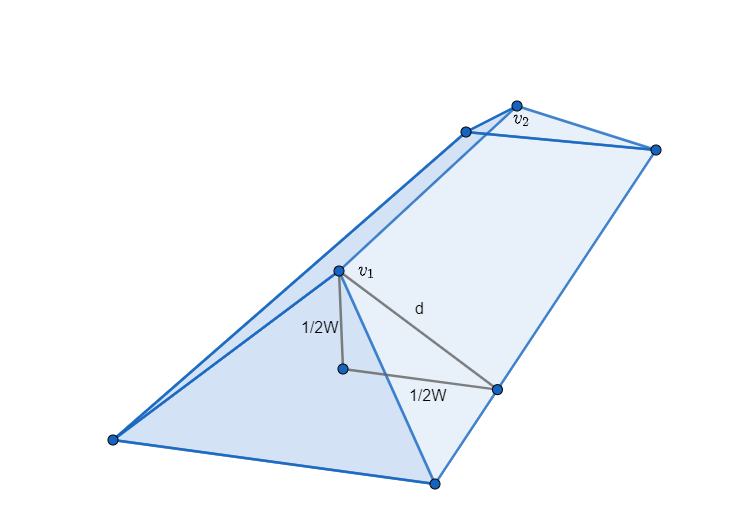
\includegraphics[scale=0.5]{roof.png} 

\section{5.8}
\begin{proposition} In a convex polygon, the first angle bisectors to meet are at adjacent vertices. 
\end{proposition}

\begin{proof}

Let $P$ be a convex polygon, and suppose by way of contradiction that there exists non-adjacent vertices $p$ and $q$ such that the angle bisectors at $p$ and $q$ intersect to form congruent edges $e_1$ and $e_2$, and where these are the shortest such edges. (This is a more precise way of saying that the angle bisectors at $p$ and $q$ intersect "first" as the textbook asks us to show).

The angle bisectors will intersect each other at an angle, pick one side of both of the angle bisectors lines such that the angle of intersection between the line segments $e_1$ and $e_2$ is convex, and call this region of the plane $S$. This region $S$ will contain some of the points of $P$. Now we can form the convex polygon $P'$, where the vertices of $P'$ are those vertices of the polygon $P$ which are contained within $S$, as well as $p$ and $q$ and the intersection of their angle bisectors. This polygon $P'$ will be convex, for we had that $p$ and $q$ were convex, and we have chosen the sides of of the angle bisectors so that the angle $e_1e_2$ is convex. \\

Since by construction $p$ and $q$ are not adjacent, there must exist some vertex $r$ on $P'$ which is also a vertex of $P$. Let $b$ be the angle bisector at $r$. Since the edges adjacent to $r$ are also part of $P$, this is also one of the angle bisectors of the original polygon $P$. Moreover, since $P'$ is convex, we must have that $r$ crosses the boundary of $P'$ exactly twice. The first time is at $r$. There must be another intersection of $r$ with the boundary. There are two cases. Either $r$ intersects with the boundary of $P$, or with the angle bisectors $e_1$ and $e_2$.\\

The first case is far less likely to happen, and I'm even suspicious of whether or not it could. I'll cover it anyway, just in case. If $b$ meets with a boundary point on an edge of $P$, it must have also crossed over another point $s$ between $p$ and $q$. In this case, the angle bisector $b$ must have crossed over some other vertex between $p$ and $q$ on the polygon $P$, call it $s$. Then the angle bisector at $s$ must also cross through $b$, and this will occur inside the polygon $P'$. The length of the resulting edges will be shorter than $e_1$ and $e_2$, so we arrive at a contradiction since in fact the angle bisectors at $r$ and $s$ meet first. (based upon an argument from angles and convexness, I am pretty sure the first case I just listed can't happen)\\


The second case is nice and concise, and in my opinion captures the essence of the proof. Suppose that $b$ meets with either $e_1$ or $e_2$. Then the resulting segment will be shorter, and the pair of bisectors $(r,q)$ or $(r,p)$ will meet before $(p,q)$. \\

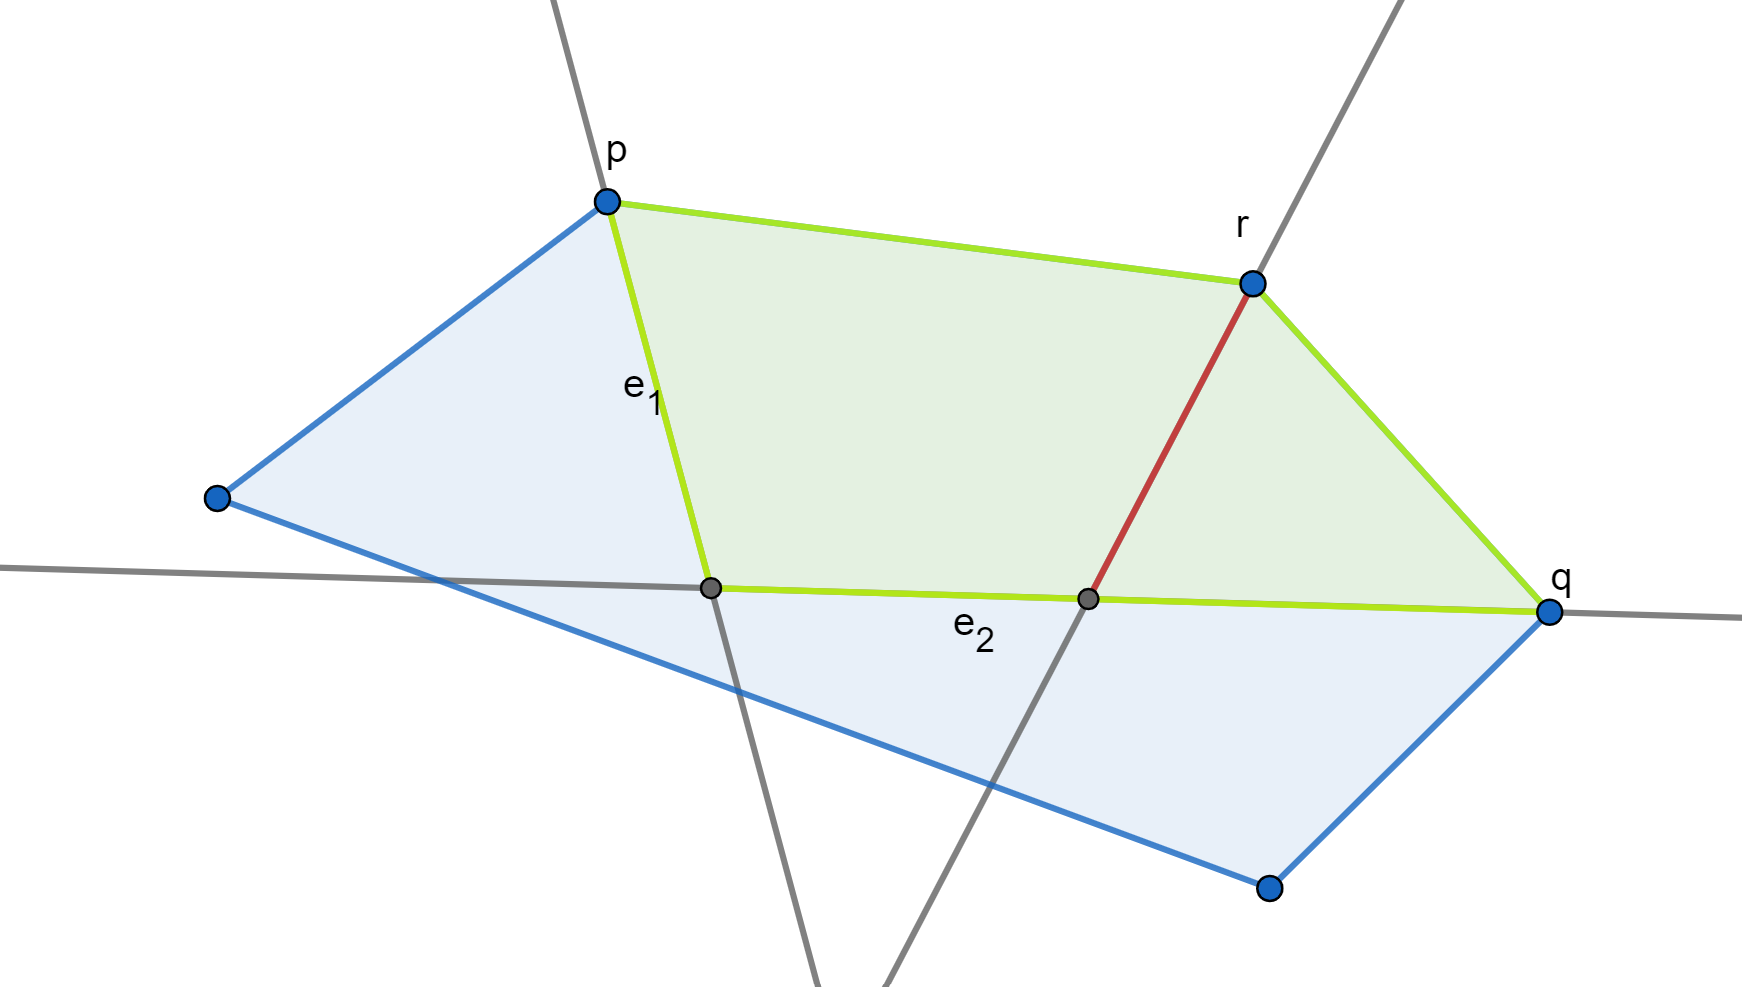
\includegraphics[scale=0.5]{proof.png} 

This concludes the proof, kind of. Unfortunately it isn't quite to my own satisfaction, but I must turn it in anyway.
\end{proof}


\section{5.22}


\begin{proposition}

Let $x$ be a point in $\R^2$. For each $n\in \N$, the minimum number of vertices in a closed polygonal curve such that the winding number of this curve at $x$ is $n$, is $3n$. By calling it the minimum, I mean that it is realized in an actual curve.

\end{proposition}

\begin{proof}

First, for $n = 1$, the smallest number of vertices required to make a polygonal curve enclose any region at all is $3$. The oriented boundary of a triangle will do, and therefore the base case holds.\\

Now suppose that the minimum number of vertices for a closed polygonal curve about $x$ with winding number $n$ about $x$ is $3n$. Certainly $n$ times looping around the boundary of a triangle enclosing $x$ will give us a winding number of $n$. Now suppose by way of contradiction that some closed polygonal curve $C$ does in fact exist in the case for $n+1$, which encloses $x$, and which has less than $3(n+1)$ vertices. Well then, if $V(C)$ denotes the number of vertices, $V(C)\le 3n + 2$. The idea is to use this to construct a curve $C'$ about $x$ with winding number $n$ and with less than $3n$ vertices. \\

While we have not rigorously defined the winding number, I suspect it could be done by showing that it is half the minimum number of points at which a line based at $x$ crosses the curve $C$. I shall assume this to be the case (of course I am thereby assuming that there \textit{is} such a minimum, which is less trivial than it seems). By our assumption that the winding number of $C$ about $x$ is $n+1$, and by this notion of the winding number, there must exist some line $l$ at $x$ which intersects $C$ $2(n+1)$ times. With respect to some sort of orientation, we can order half these $n+1$ points of intersection from first to last. Let $t_1,\dots, t_{n+1}$ be the points of intersection in order.  Let $v_n$ be the vertex of the curve directly before $v_i$, and let $v_f$ be the vertex of the curve directly after $t_{n+1}$. Connecting these vertices, we obtain a new closed polygonal curve $C'$ with winding number at least $1$, and whose vertices are all vertices of $C$. Since the line segment containing $v_i$ and $t_n$ can only cross $l$ once, it follows that the vertex direct after $t_{n-1}$ is not $v_i$. From this it follows that we can safely remove all of the last bit of the curve $C'$ from $C$, all the while only decreasing the winding number by $1$. Finally, connecting back the vertex directly before $t_{n-1}$ to the first vertex, we form a new curve $C''$. Since we have removed three vertices and gained none in constructing $C''$, we now have a curve with winding number $n$ about $x$, but with $3n-1$ vertices. This contradicts the induction hypothesis. \\


While my proof is not as air tight as I would like, I do think a rigorous proof would be something to this effect.
\end{proof}

\section{Problem (a)}

While I have not got a proof, I think that the maximum number of vertices achievable in the Minkowski sum of two pentagons is 14. Here are the pentagons I am summing in creating this example:


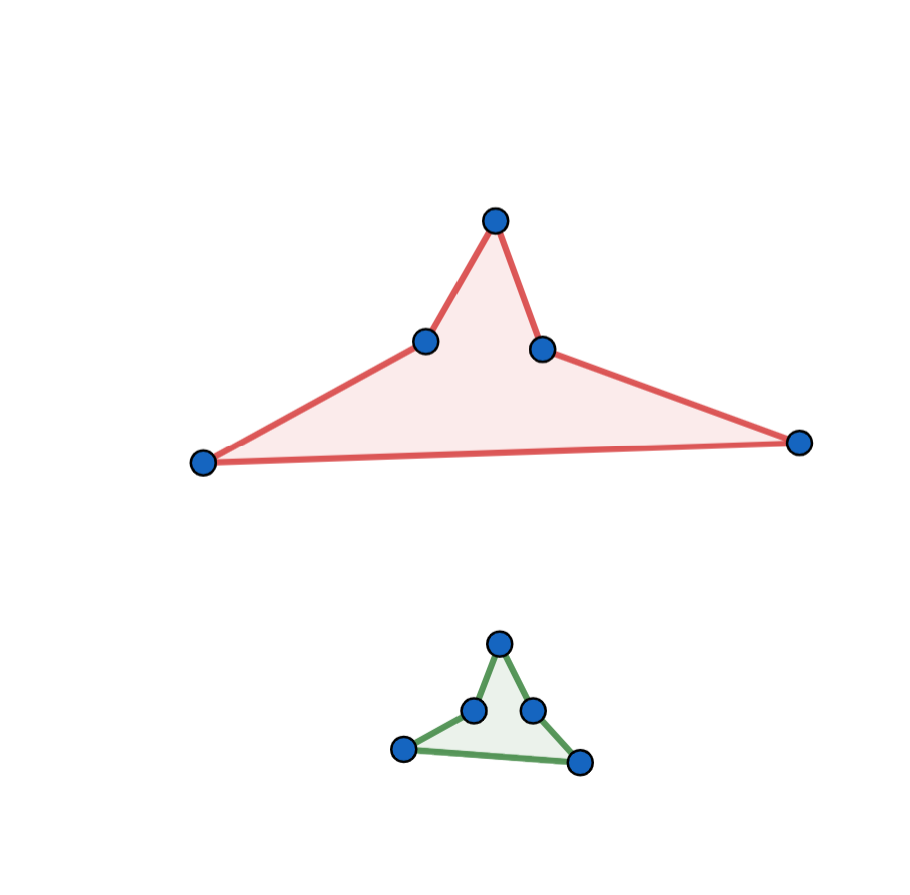
\includegraphics[scale=1]{polygons.png} 

We can construct the Minkowski sum by fixing 

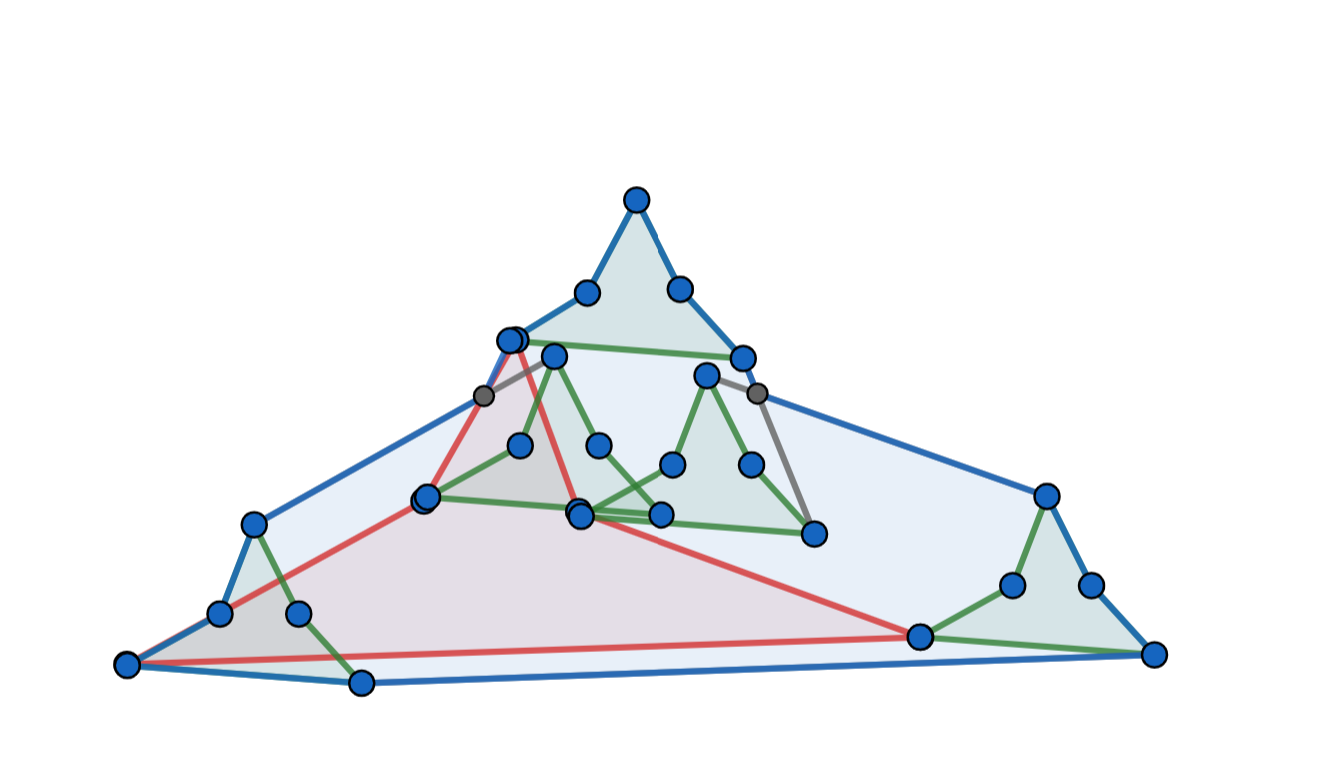
\includegraphics[scale=1]{minkowski_sums.png}.


\section{Problem (b)}

\begin{proposition} The edges Gabriel graph of a point set $S$ are the edges of the Delauney triangulation which cross their associated Voronoi edge. 
\end{proposition}

\begin{proof}

First, I will show that if for points $p,q\in S$, $pq$ does not cross $V(p,q)$, then this edge is not a Gabriel edge. Then I will show that if $pq$ is not a Gabriel edge, then $pq$ doesn't cross $V(p,q)$. Since the Delaunay triangulation and the Voronoi diagram (as graphs) are dual to each other, the edges of the Dalaney triangulation are in one to one correspondence with crossings of the Voronoi edges. 

Suppose that $pq$ does not cross $V(p,q)$. Extend $V(p,q)$ to obtain the perpendicular bisector $B(p,q)$. Clearly $pq$ crosses $ B(p,q) $ at exactly one point, $m$. But $m$ cannot be in $V(p,q)$, for otherwise $pq$ would cross $V(p,q)$. Hence $m$ cannot be in the Voronoi region of $p$ and $q$. The Voronoi regions cover the plane, hence $m$ lies in some other Voronoi region, $V(x)$, and $m$ must be strictly closer to $x$ than to $p$ and $q$. Hence $x$ is interior to the circle of radius $pm$ centered at $m$. By definition of a Gabriel edge, $pq$ cannot be a Gabriel edge.

Now suppose conversely that $ pq $ is not a Gabriel edge. Since $pq$ is not a gabriel edge, some other point of the point set, say $x$, lies interior to the circle of diameter $pq$ centered at the midpoint, $m$. Since $m$ lies on the perpendicular bisector to $pq$, if $pq$ crosses $V(p,q)$, it ought to be there. But since $x$ is interior to the circle of diameter $pq$ (and hence radius $pm$) centered at $m$, $m$ is \textit{strictly} closer to $x$ than to either of $p$ and $q$. Hence $m$ is in the Voronoi region of $x$, and not in the Voronoi region of $p$ or $q$. From this it follows that $m$ is not on the boundary of $V(p)$ nor of $V(q)$, and hence that $m$ is not on $V(p,q)$. Since $V(p,q)$ is a subset of the perpendicular bisector of $pq$, and since $pq$ crosses its perpendicular bisector at only one point $m$, which is not in $V(p,q)$, $pq$ cannot cross $V(p,q)$.

This concludes the proof.


\end{proof}



\end{document}